\chapter{The Groth Strip with Dutch LOFAR}\label{section.EGS.lowres}
\minitoc
% % % % % % % % % % % % % % % % % % % % % % %
\section{Aims \& Methodology}

\pg
In this section, we describe the work done to make a wide-field image of the entire LOFAR primary beam, centred on EGS. A large-field, image of this field has never yet been made at such low frequencies. Due to technical limitations, the maximum attainable image size (in terms of number of pixels) will limit resolution to about $5''$. As such, the international stations are not used for this part of the project.
A more complete sky model can be created from this image, and %, allowing for one last round of self-calibration on the 3C295 high-resolution model. 
bright out-of-field sources can be subtracted from high-resolution images of the Extended Groth Strip so that their sidelobe emission do not contaminate the final images. To achieve this, we require direction-dependent calibration. Because we do not use the international LOFAR stations, we do not need a high-resolution model of 3C295. %  This ensures that we do not ``hard-set" errors in our high-resolution model caused by other sources in the field. 

\pg
We aim to achieve a sensitivity of a few hundreds of $\mu$Jy using visibilities recorded between $110-180$ MHz. This corresponds to a sensitivity of $\sim20$ $\mu$Jy at 1.4 GHz for typical synchrotron radio sources, which have spectral indices of $\alpha\sim -0.7$ (where $S_\nu \propto \nu^\alpha$). Reaching this sensitivity goal over the full LOFAR primary beam requires direction-dependent calibration.
Our methodology is therefore to calibrate the full LOFAR bandwidth using the LOFAR Surveys KSP pipeline, which performs a facet-based direction-dependent calibration. We then perform source analysis on the most interesting objects in the field, using ancillary data from NVSS \citepads[NRAO VLA Sky Survey, ]{1998AJ....115.1693C}, SDSS \citepads[Sloan Digital Sky Survey, ]{2000AJ....120.1579Y} and WISE \citepads{2010AJ....140.1868W} surveys and cross-referenced using SIMBAD \citepads{2000A&AS..143....9W}. Overlays for those sources will be shown in \cref{sec.lowresEGS.overlays}.


% % % % % % % % % % % % % % % % % % % % % % %
\section{Data Reduction}


\subsection{Data \& Observation Properties}
\pg
The dataset used for this PhD project is part of the LOFAR Surveys KSP Tier-1 survey, which consists of a number of 8-hour pointings covering as much of the sky visibile to LOFAR as possible. We analyse one of these pointings, an observation performed on the 28th of August 2014 and centred on the Extended Groth Strip. As part of the Tier-1 survey, it is an 8-hour-long observation. We limit ourselves to analysing only the HBA observation, meaning that we use 365 sub-bands which sample a total bandwidth of 110-182 MHz. We use all Core and Remote LOFAR stations, as well as some of the International stations which were online at the time (specifically the German stations 1-5 and 7, along with the Swedish and the British station).

\pg
The observation is centred on the EGS, and not on 3C295. This means that our calibrator source is not at phase centre, which can potentially introduce problems. Thankfully, new developments in imaging \citepads{2017arXiv171202078T} ensure that the direction-dependent PSF (one of the problems introduced by an off-centre calibrator) is properly modeled and corrected for. This means that direction-independent calibration will be exactly correct in the direction of 3C295, and a good model of this source can be made.

\pg
The data was acquired through the LOFAR Long-Term Archive, and is thus pre-processed and flagged for RFI using the standard tools (NDPPP\citetads{2018ascl.soft04003V} and AOFlagger \citetads{2010ascl.soft10017O}, respectively). The next step is therefore to calibrate the data.

\subsection{Reducing the Data}

\pg
Reducing LOFAR data is a complex business for a number of reasons. When seeking to make high-fidelity, wide-field images, the need to minimise decorrelation (cf. \cref{section.RIME.TimeDep.Decoherence}) means that data can only be averaged with care. As visibilities are averaged in time and frequency\footnote{Provided that simple averaging is performed; the use of baseline-dependent window functions can alleviate this effect to some extent}, the relative contribution of signal picked up on longer baselines from sources far from the observation centre is decreased. This translates to a blurring of sources as distance from phase centre increases.

\pg
What's more, antenna gains can vary over short durations or show peculiar spectral behaviour. Even if interferometric data were averaged massively using baseline-dependent window functions, information on this underlying gain behaviour would be lost - this means that averaging data to reduce its size (and associated reduction wall time) is a risky proposition.

\pg
As such, we seek to reduce an eight-hour LOFAR HBA observation, averaged down to 1 measurement per second and per 24 kHz\footnote{This is the bandwidth for each channel of our observation.}. This corresponds to a total of 7 terabytes of raw data: 2920 frequency measurements each second, for 28800 second, of 4 correlations, for each baseline. The observation mode used was HBA\textunderscore DUAL\textunderscore INNER, in which all Dutch stations operate with 24 of their 48 tiles, and these substations are then correlated separately with the rest of the array. This was chosen because this configuration does not negatively impact the array density of short baselines (allows for better sensitivity to, and thus recovery of, diffuse emission), nor does it introduce the calibration difficulties that non-uniform beams would cause.

\pg
The calibration strategy consists of a first round of direction-independent calibration followed by direction-dependent self-calibration. In effect, we use the following RIME:
\begin{equation}
\Vis_{pq} = \Gjones_p \bigg( \sum_s \Ejones_{sp} \Kjones_{sp} \Bmatrix_{s} \Kjones_{sq}^H \Ejones_{sq}^H \bigg) \Gjones_q^H
\end{equation}
which is the same as \cref{eq.multiple.source.RIME}. To account for the faceting explicitly, we can write:
\begin{equation}
\Vis_{pq} = \Gjones_p \sum_{\Omega}\bigg( \sum_{s\in\Omega} \Ejones_{sp} \Kjones_{sp} \Bmatrix_{s} \Kjones_{sq}^H \Ejones_{sq}^H \bigg) \Gjones_q^H
\end{equation}
where $\Omega$ indices denote different facets, and $s$ indices denote individual sources. Each source in a given facet is assumed to have similar direction-dependent gains, and their cumulative signal-to-noise allows for better estimations of this direction-dependent gain than would be possible if solving for each source individually. Thus:
\begin{equation}
\Vis_{pq} = \Gjones_p \sum_{\Omega}\bigg( \sum_{s\in\Omega} \Ejones_{\Omega p} \Kjones_{sp} \Bmatrix_{s} \Kjones_{sq}^H \Ejones_{\Omega q}^H \bigg) \Gjones_q^H
\end{equation}

\pg
We begin with direction-independent calibration to find an estimate of $\Gjones_p\forall p$. This first step is done because this part of the Jones chain is the same throughout the sky, and its inverse solution can therefore be applied directly to the visibilities as follows:
\begin{align}
\Vis_{pq}^\mathrm{corr} &= \Ghatjones_p^{-1} \Vis_{pq} \left( \Ghatjones_q^H \right)^{-1}\\
						&= \Ghatjones_p^{-1}\Gjones_p \sum_{\Omega}\bigg( \sum_{s\in\Omega} \Ejones_{\Omega p} \Kjones_{sp} \Bmatrix_{s} \Kjones_{\Omega q}^H \Ejones_{sq}^H \bigg) \Gjones_q^H \left( \Ghatjones_q^H \right)^{-1}
\end{align}
In so doing, we assume that $\left(\Ejones_{sp}\forall s,p\right) =1$ when solving for $\Ghatjones$. In general, this is of course invalid. For the calibrator source, however, we have $Ejones_{sp} =1 \forall p$ by construction. Because we can choose the calibrator source, the presence of a sufficiently bright source (in our case, an unresolved 3C295) will give extremely good estimations of $\Gjones$. We then have $\Ghatjones_p^{-1}\Gjones_p\sim 1$, and
\begin{align}
\Vis_{pq}^\mathrm{corr} &\sim \sum_{\Omega}\left( \sum_{s\in\Omega} \Ejones_{\Omega p} \Kjones_{sp} \Bmatrix_{s} \Kjones_{sq}^H \Ejones_{\Omega q}^H \right)
\end{align}
and direction-dependent calibration then consists of solving for $\Ehatjones_{\Omega p} = \Ghatjones_p^{-1}\Gjones_p\Ejones_{\Omega p} \sim \Ejones_{\Omega p}$ for all facets.

\pg
Direction-independent calibration is done with Prefactor \citepads{2016ApJS..223....2V}, using an initial sky model generated using the VLSSr \citepads[VLA Low-frequency Sky Survey - redux, ]{2012RaSc...47.0K04L}, WENSS \citepads[WEsterbork Northern Sky Survey]{1997A&AS..124..259R} and the NVSS \citepads[NRAO VLA Sky Survey, ]{1998AJ....115.1693C}, with 3C295 dominating the model. This model also serves as the initial model for the direction-dependent facet-based self-calibration on the corrected visibilities, performed using the killMS-DDF pipeline \citepads{2017A&A...598A.104S}. The quality-based weighting scheme discussed in \cref{chapter.paper} was used to improve self-calibration convergence and the final image.

\pg
Direction-dependent calibration was required, as the field of view is large enough that differential ionospheric errors are introduced as a function of direction: the signal from different sources cross different sections of the ionosphere, and the actual gains for these sources are thus different from the gains for the calibrator. They must thus be solved for individually. Assuming that the scale of ionospheric change is of the order of a degree (which is what is observed empirically), then a facet-based approach will give a ``good enough" result for most of the field. The direction-dependent calibration consisted of a physics-based approach, solving for XX and YY correlations along with a rotation matrix simulating differential Faraday rotation. These gain solutions were then smoothed in time and frequency to provide a time-independent, frequency-dependent amplitude solution for each station. The full LOFAR bandwidth is large enough to allow for Clock/TEC separation, which consists of explicitly modeling the two direction-independent phenomena which dominate in the gain's spectral structure. The clock difference between stations\footnote{Each station has a relatively-accurate clock associated with it, save for the Superterp stations which all share a single clock. Like all clocks, they have finite accuracy, and desynchronisation errors thus creep in over time.} introduces a phase error proportional to $\nu$, while differences in Total Electron Content (TEC) along the line of sight of different stations introduce a phase error inversely proportional to $\nu$. With sufficient spectral coverage, these two effects can therefore be separated and modeled individually, thereby improving the phase solution conditioning. 


\begin{figure}[h!]
\centering
\includegraphics[width=0.95\textwidth]{images/{image_full_ampphase_di_m.NS_Smooth.noise01.fitsnoisemap.facets}.png}
\caption{\label{fig.EGS.widefield.regions} Facet distribution for the full direction-dependent calibrated image of the LOFAR primary beam. Image made without international stations. Note that 3C295 is easily found in the image: the dominant calibration artefacts are centred around it.}
\end{figure}

\pg
The direction-dependent calibration was done using 121 facets, spread as shown in \cref{fig.EGS.widefield.regions}. Some facets converge faster or better than others, and so artefacts due to direction-dependent effects may remain in certain areas of the image but not others. Calibration is done solving for full, complex Jones matrices, rather than a physics-based or diagonal-and-rotation matrix.
The final image was imaged with a $uv$-cut, keeping only baselines longer than 100m. This is because shorter baselines were not used during calibration, and so discarded for imaging. The image resolution is $1.5''$, and the image was created using both quality-based weighting schemes and Briggs weighting, with a Briggs factor of $-0.5$. This means that the imaging was skewed slightly in favour of uniform weighting (weighting visibilities by local $uv$-density) rather than natural weighting (same weight for all visibilities). Imaging and calibration were done using the LOFAR beam model used in AWImager \citepads{awimager}, so the image gives integrated flux values rather than apparent flux values. Deconvolution was performed on the full bandwidth\footnote{This improves the conditioning of the imaging inverse problem, as it means that bright structure present across the full band (e.g. hotspots) can be deconvolved with the smaller PSF peak of the hightest-frequency band.} using SSD-clean with an external mask.

\begin{figure}[h!]
\centering
\begin{subfigure}{.48\textwidth}
\resizebox{\hsize}{!}{\includegraphics{images/{image_dirin_SSD_m_c_di_m.int.restored.fits}.png}}
\caption{\label{image.egs.widefield.noddsc} LOFAR wide-field image cutout, calibrated with the initial sky model and no direction-dependent Jones terms.}
\end{subfigure}
\hfill
\begin{subfigure}{.48\textwidth}
\resizebox{\hsize}{!}{\includegraphics{images/{image_full_ampphase_di_m.NS.app.restored.fits}.png}}
\caption{\label{image.egs.widefield.doddsc} LOFAR wide-field image cutout, self-calibrated from \cref{image.egs.widefield.noddsc} with direction-dependent Jones terms.}
\end{subfigure}
\caption{\label{image.egs.widefield.ddsc} Wide-field image cutouts of the full primary beam, centred on the EGS, before and after selfcal.}
\end{figure}

\pg
Direction-dependent self-calibration dramatically improves the noise level in the final image, as shown in \cref{image.egs.widefield.ddsc}. Note that not only do artefacts centred on 3C295 (which dominate the noise level in \cref{image.egs.widefield.noddsc}) decrease dramatically, but many of the "diffuse" sources in the field also seem to disappear: this is because their associated artefacts also decrease dramatically, and only physical emission remains. % Because this is a very large and high-resolution image, this means that most of these sources end up occupying a single pixel of the png cutout, and so appear to disappear. 

\begin{figure}[h!]
\centering
\begin{subfigure}{.48\textwidth}
\resizebox{\hsize}{!}{\includegraphics{images/{widefield.DI}.png}}
\caption{\label{image.egs.widefield.noddsc.zoom} LOFAR wide-field image cutout, calibrated wtih the initial sky model and no direction-dependent Jones terms.}
\end{subfigure}
\hfill
\begin{subfigure}{.48\textwidth}
\resizebox{\hsize}{!}{\includegraphics{images/{widefiled.DD}.png}}
\caption{\label{image.egs.widefield.doddsc.zoom} LOFAR wide-field image cutout, self-calibrated from \cref{image.egs.widefield.noddsc} with direction-dependent Jones terms.}
\end{subfigure}
\caption{\label{image.egs.widefield.ddsc.zoom} Cutouts of smaller regions of \cref{image.egs.widefield.ddsc}.}
\end{figure}

\pg
These sources nevertheless remain in the field, as shown in \cref{image.egs.widefield.ddsc.zoom}. Note that the noise level is not constant throughout the image: this is because the array is not uniformly sensitive to the entire sky, but has a specific beam response. Correcting for this beam response in the image-plane gives integrated flux rather than apparent flux. A full catalogue of the sources in this image is given in \cref{appendix.widefield.catalog}, \cref{widefield.survey.catalog} % gives rise to this effect. 

\pg
Finally, the quality-based weighting schemes developed in \cref{chapter.paper} were applied throughout this procedure. Noise maps made with and without the weighting scheme are shown in \cref{image.egs.widefield.weights}. A few things are important to note in this comparison. Firstly, the weighting schemes decrease the noise by a factor of $\sim10$: for the noise-map to be visible without weighting schemes, the contrast of the weighted image needed to be pushed way low. For reference, \cref{image.egs.widefield.weighted} is the same image (albeit without the facets shown explicitly) as \cref{fig.EGS.widefield.regions}. The noise distribution is more clearly visible in that figure. Relatedly, by comparing that image and \cref{image.egs.widefield.noweights}, we note that the unweighted image has a different noise per facet, unlike the weighted image. This is due to the fact that a single visibility will be calibrated better or worse depending on the facet which the flux model is used for calibration. It is no coincidence that the facet containing 3C295 is the only one with a noise even remotely comparable to the weighted image's: it is the facet with the best signal-to-noise. This becomes significant when taking into account the fact that the last 2 hours of this observation are much noisier than the first 6: the quality-based weights will decrease their overall contribution \textit{throughout the image}, whereas not using them will lead to different facets having stronger or lesser contributions from these noisy visibilities - and therefore different noise levels. This is also why fringes can clearly be seen in some facets: a single visibility (or a set of a few visibilities) are particularly badly-calibrated, and the associated fringe dominates in the facet. Linking back to \cref{chapter.paper}, because we have a gain solution per visibility \textit{and per facet}, we have one noise-PSF per facet; this suggests that the quality-based weighting scheme could likely be extended to a direction-dependent formalism.

\begin{figure}[h!]
\centering
\begin{subfigure}{.65\textwidth}
\resizebox{\hsize}{!}{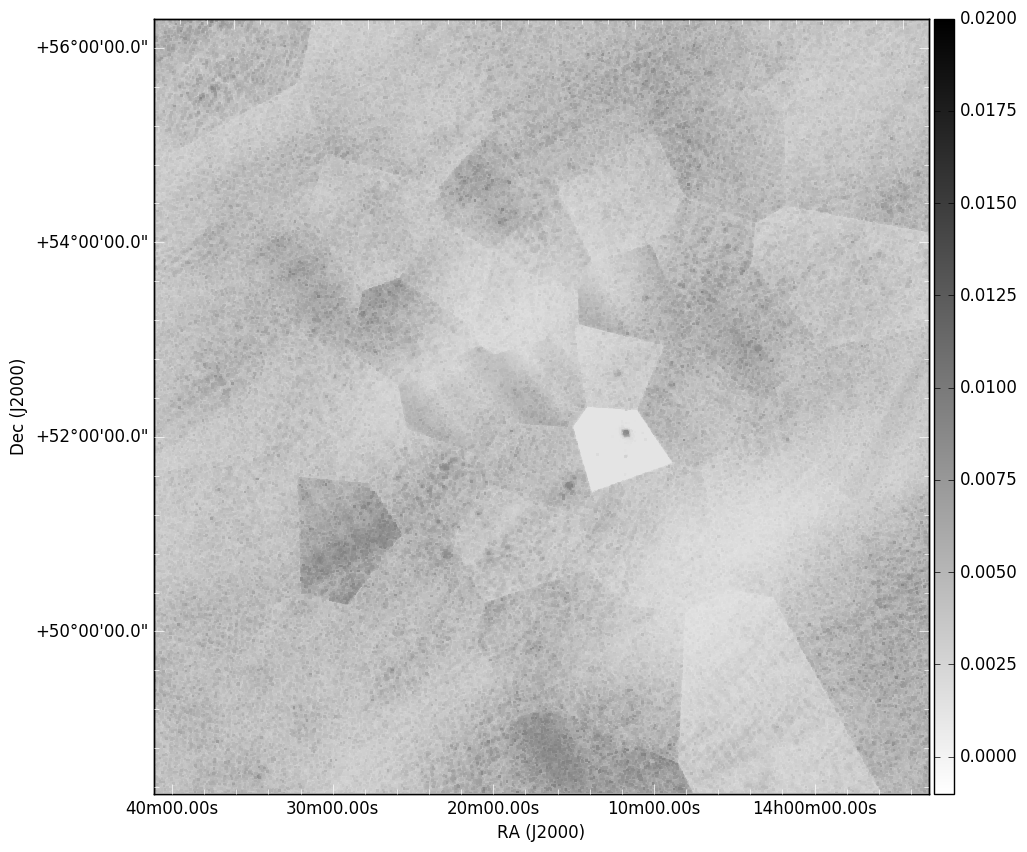
\includegraphics{images/{./image_full_ampphase_di_m.NS_Smooth_noW.noise01.fitsnoisemap.weights.compare}.png}}
\caption{\label{image.egs.widefield.noweights} OFAR wide-field image cutout, self-calibrated from \cref{image.egs.widefield.noddsc} with direction-dependent Jones terms, made without using quality-based weights.}
\end{subfigure}
\hfill
\begin{subfigure}{.65\textwidth}
\resizebox{\hsize}{!}{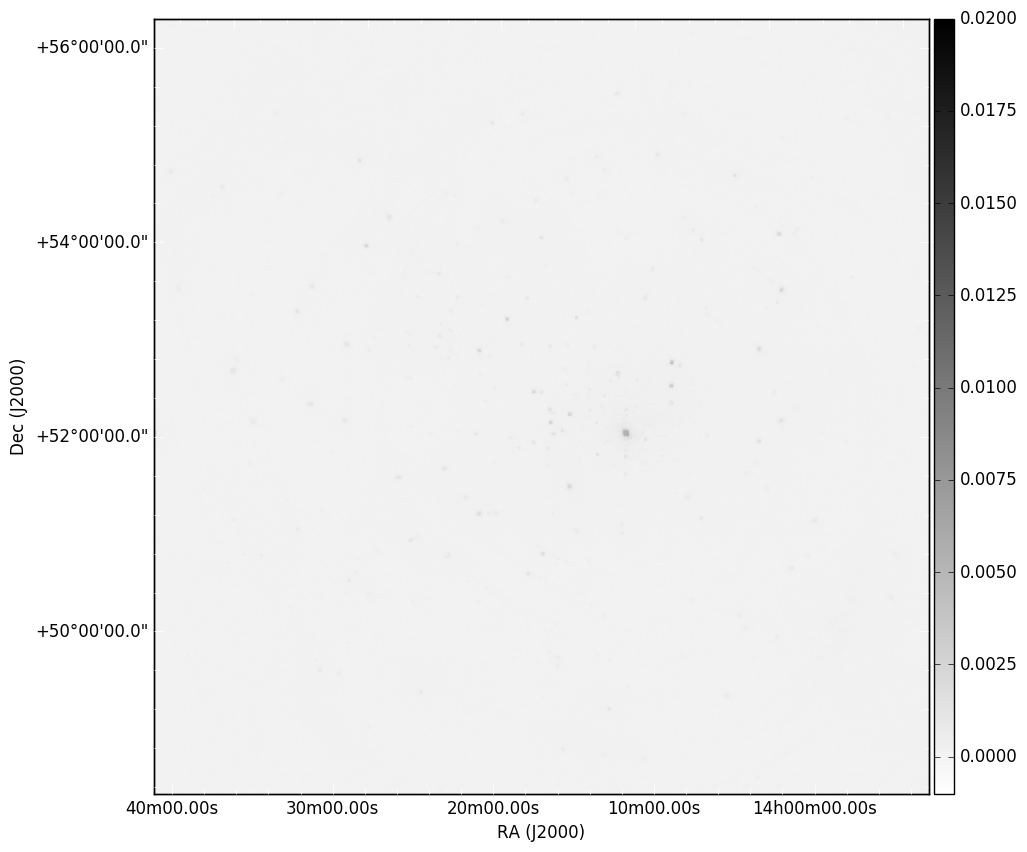
\includegraphics{images/{./image_full_ampphase_di_m.NS_Smooth.noise01.fitsnoisemap.weights.compare}.png}}
\caption{\label{image.egs.widefield.weighted} LOFAR wide-field image cutout, self-calibrated from \cref{image.egs.widefield.noddsc} with direction-dependent Jones terms, made with quality-based weights.}
\end{subfigure}
\caption{\label{image.egs.widefield.weights} Impact of quality-based weighting scheme on the final image.}
\end{figure}


\clearpage

% % % % % % % % % % % % % % % % % % % % % % %
\section{Overlays \& Images}\label{sec.lowresEGS.overlays}

%\subsection{Selected Sources}

\pg
We select 12 sources in the wide-field image, which is shown in \cref{plot.EGS.lofar.widefield}. Our selection is primarily based on whether sources have interesting or peculiar diffuse emission, though some are chosen for being particularly classic examples of radio galaxies. We scan the image from south to north and east to west (scanning upwards then shifting to the right in the image). The positions of the brightest sources ($>1$Jy)are given in \cref{table.egs.sources}.


\begin{figure}[h!]
\centering
\includegraphics[width=0.95\textwidth]{images/{lofar.widefield}.png}
\caption{\label{plot.EGS.lofar.widefield} Full direction-dependent calibrated image of the LOFAR primary beam, centred on the EGS. Image made without international stations.}
\end{figure}

\begin{table}[h!]
\begin{tabular}{ccccc}
Name    & RA [hms]    & Dec [dms]   & Likely Association            & LOFAR thumbnail \\\hline
EGS-1   & 14:37:39.53 & 53:36:31.24 & NVSS Radio Galaxy             & \cref{fig.egs1.lofarim} \\
EGS-2   & 14:35:27.84 & 55:07:56.32 & Radio Galaxy in Cluster       & \cref{fig.egs2.lofarim} \\ 
EGS-3   & 14:29:34.13 & 54:43:46.93 & Radio Galaxy in Cluster       & \cref{fig.egs3.lofarim} \\
EGS-4   & 14:31:36.62 & 52:27:33.75 & Radio galaxy, $z=.292$        & \cref{fig.egs4.lofarim} \\
EGS-5   & 14:29:48.89 & 51:10:30.52 & Lobes matched individually    & \cref{fig.egs5.lofarim} \\
EGS-6   & 14:26:04.09 & 51:29:35.07 & One lobe matched individually & \cref{fig.egs6.lofarim} \\
EGS-7   & 14:17:55.58 & 50:08:01.75 & Radio galaxy, $z=.186$        & \cref{fig.egs7.lofarim} \\
EGS-8   & 14:14:40.42 & 51:17:41.00 & Radio galaxy, $z$ unknown     & \cref{fig.egs8.lofarim} \\
EGS-9   & 14:11:36.43 & 52:54:25.53 & Galaxy cluster, $z=.525$      & \cref{fig.egs9.lofarim} \\
EGS-10  & 14:07:09.90 & 55:04:22.23 & Galaxy cluster, $z=.250$      & \cref{fig.egs10.lofarim} \\
EGS-11  & 14:03:16.00 & 51:43:35.23 & Lobes matched individually    & \cref{fig.egs11.lofarim} \\
EGS-12  & 14:02:43.49 & 51:03:14.69 & Radio Galaxy in Cluster       & \cref{fig.egs12.lofarim} \\
\end{tabular}
\caption{\label{table.egs.sources} Table recapitulating the names, positions and likely associations of all 12 chosen sources in the primary beam. These sources were primarily chosen because they had peculiar or interesting diffuse emission. The associated LOFAR image thumbnails are also given for reference.}
\end{table}

\pg
\cref{table.egs.sources} also gives the likely associations for each chosen EGS source, giving redshift information when available. The analysis here is done by hand using NED (\href{https://ned.ipac.caltech.edu/}{NASA/IPAC Extragalactic Database (NED)}), Simbad (\href{http://simbad.u-strasbg.fr/simbad/}{
operated at CDS, Strasbourg}) and the associated catalogues and papers, often accessible through ADS (\href{http://adsabs.harvard.edu/}{SAO/NASA Astrophysics Data System (ADS)}). Such an artisanal approach is suitable for the analysis of a dozen sources, but quickly becomes intractable. % Ideally, one would rely on automated matching between sources extracted from the widefield image and complete catalogues at other wavelengths: this would allow the matching of hundreds of sources in the time it took to analyse 12.
Since source analysis is but a happy byproduct of our primary science aim, this was not done here, but would be a promising avenue of future work.

\pg
For each source, we show four images: a cutout of the LOFAR image around the source, an SDSS cutout of the same area with the LOFAR image superimposed as an overlay, the same SDSS cutout with an NVSS image overlayed, and finally the same SDSS image again with a WISE image overlay. The first image aims to show why the source was selected. The second shows optical counterparts to LOFAR emission. The third serves to check whether we pick up similar structure and emission in NVSS images as the LOFAR wide-field image. Note that the NVSS images are at a much lower resolution, but can be a useful way to ensure that we are not choosing artefacts or spurious emission as sources to investigate. Finally, the WISE overlay attempts to see whether infrared emission can be associated to these sources. Note that the sensitivity of SDSS images are not homogeneous, as not all patches of the sky have received the same coverage. 

%\subsection{Images \& Cross-matching}

\clearpage
\subsubsection{EGS-1}


\begin{figure}[h!]
\centering
\begin{subfigure}{.48\textwidth}
\resizebox{\hsize}{!}{\includegraphics{images/{egs1.LOFARegs}.png}}
\caption{\label{fig.egs1.lofarim} Cutout of our LOFAR wide-field image centred on EGS-1.}
\end{subfigure}
\hfill
\begin{subfigure}{.48\textwidth}
\resizebox{\hsize}{!}{\includegraphics{images/{egs1.lofar}.png}}
\caption{\label{fig.egs1.sdss.lofoverlay} SDSS image of EGS-1, with \cref{fig.egs1.lofarim} as an overlay.}
\end{subfigure}
\hfill
\begin{subfigure}{.48\textwidth}
\resizebox{\hsize}{!}{\includegraphics{images/{egs1.nvss}.png}}
\caption{\label{fig.egs1.sdss.nvssoverlay} Same image as \cref{fig.egs1.sdss.lofoverlay}, with NVSS overlay.}
\end{subfigure}
\hfill
\begin{subfigure}{.48\textwidth}
\resizebox{\hsize}{!}{\includegraphics{images/{egs1.Wise3.4}.png}}
\caption{\label{fig.egs1.sdss.wiseoverlay} Same image as \cref{fig.egs1.sdss.lofoverlay}, with WISE overlay.}
\end{subfigure}
\caption{\label{fig.egs1} Images \& Overlays for EGS-1.}
\end{figure}

\pg
EGS-1 was selected from the wide-field LOFAR image because it showed interesting diffuse structure. It does not seem to match up to any optical source, nor does it match an infrared source. EGS-1 therefore seems to be best identified as a low-frequency counterpart to NVSS J143706+533225. Its shape seems to include two jets, one much brighter than the other, but both visible in \cref{fig.egs1.lofarim}. This is congruent with a radio galaxy with one Doppler-boosted jet. The absence of an optical counterpart could be due to dust extinction or to insufficient sensitivity. 

\clearpage
\subsubsection{EGS-2}

\begin{figure}[h!]
\centering
\begin{subfigure}{.48\textwidth}
\resizebox{\hsize}{!}{\includegraphics{images/{egs2.LOFARegs}.png}}
\caption{\label{fig.egs2.lofarim} Cutout of our LOFAR wide-field image centred on EGS-2.}
\end{subfigure}
\hfill
\begin{subfigure}{.48\textwidth}
\resizebox{\hsize}{!}{\includegraphics{images/{egs2.lofar}.png}}
\caption{\label{fig.egs2.sdss.lofoverlay} SDSS image of EGS-2, with \cref{fig.egs2.lofarim} as an overlay.}
\end{subfigure}
\hfill
\begin{subfigure}{.48\textwidth}
\resizebox{\hsize}{!}{\includegraphics{images/{egs2.nvss}.png}}
\caption{\label{fig.egs2.sdss.nvssoverlay} Same image as \cref{fig.egs2.sdss.lofoverlay}, with NVSS overlay.}
\end{subfigure}
\hfill
\begin{subfigure}{.48\textwidth}
\resizebox{\hsize}{!}{\includegraphics{images/{egs2.Wise3.4}.png}}
\caption{\label{fig.egs2.sdss.wiseoverlay} Same image as \cref{fig.egs2.sdss.lofoverlay}, with WISE overlay.}
\end{subfigure}
\caption{\label{fig.egs2} Images \& Overlays for EGS-2.}
\end{figure}


\pg
EGS-2 was selected from the wide-field LOFAR image because of the interestingly turbulent morphology of its northern jet, and extended diffuse emission. 
A bright optical source lies very close to the mid-point of EGS-2. This source - 2MASX J14352846+5507519\footnote{\url{http://simbad.u-strasbg.fr/simbad/sim-id?Ident=\%40499314&Name=2MASX\%20J14352846\%2b5507519&submit=submit}} - is the brightest galaxy in a cluster. It lies at a redshift of 0.13985 \citepads{2013yCat.5139....0A}. Furthermore, there is an NVSS source which seems to nicely overlap the EGS-2: NVSS J143527+550756 \citepads{1998AJ....115.1693C}. These two sources do not seem to be associated in the literature, though 2MASX J14352846+5507519 is associated with VLSS 1435.4+5507 - a likely counterpart to the NVSS association. These are thus likely to all be the same object.

\pg
The northern edge of EGS-2's upper jet has interesting morphology: if EGS-2 is indeed associated to the brightest galaxy in the cluster, then this morphology is likely due to differing densities of the intercluster and intracluster media, which the jets will penetrate and interact with in different ways. As ever, because this source lies far from the observation pointing, the sensitivity and calibration are not optimal for analysis: further pointings on EGS-2 might be required to achieve the signal-to-noise required to extract useful information, especially using international LOFAR.

\subsubsection{EGS-3}


\begin{figure}[h!]
\centering
\begin{subfigure}{.48\textwidth}
\resizebox{\hsize}{!}{\includegraphics{images/{egs3.LOFARegs}.png}}
\caption{\label{fig.egs3.lofarim} Cutout of our LOFAR wide-field image centred on EGS-3.}
\end{subfigure}
\hfill
\begin{subfigure}{.48\textwidth}
\resizebox{\hsize}{!}{\includegraphics{images/{egs3.lofar}.png}}
\caption{\label{fig.egs3.sdss.lofoverlay} SDSS image of EGS-3, with \cref{fig.egs3.lofarim} as an overlay.}
\end{subfigure}
\hfill
\begin{subfigure}{.48\textwidth}
\resizebox{\hsize}{!}{\includegraphics{images/{egs3.nvss}.png}}
\caption{\label{fig.egs3.sdss.nvssoverlay} Same image as \cref{fig.egs3.sdss.lofoverlay}, with NVSS overlay.}
\end{subfigure}
\hfill
\begin{subfigure}{.48\textwidth}
\resizebox{\hsize}{!}{\includegraphics{images/{egs3.Wise3.4}.png}}
\caption{\label{fig.egs3.sdss.wiseoverlay} Same image as \cref{fig.egs3.sdss.lofoverlay}, with WISE overlay.}
\end{subfigure}
\caption{\label{fig.egs3} Images \& Overlays for EGS-3.}
\end{figure}

\pg
EGS-3 is one of the most impressive sources in the primary beam. It has very complex diffuse structure. It almost certainly consists of two jets, though the interactions of these jets with the neighbouring medium must be complex indeed. From \cref{fig.egs3.sdss.nvssoverlay}, one can see that the emission can be successfully matched to no less than two individual NVSS sources. In other words, if those NVSS sources are linked to the LOFAR source - and given their spatial distribution, they almost certainly are - then they are two components of a single, deeper structure. The infrared image tells us very little.

\pg
Note that an optical source lies along the line linking the two diffuse poles of EGS-3: this source is SDSS J142933.44+544335.2, the brightest galaxy in a cluster. If EGS-3 is a radio galaxy with jet emission, which it almost certainly is (the rough symmetry of the two ``cotton balls" on either side of a ``rod"-like component strongly indicate that this is a very warped jet), then its optical emission must lie somewhere within the ``rod". That this emission would be associated with violent interactions between jet-accelerated particles and ambiant inter-cluster and intra-cluster media seems likely: it would explain the complex, turbulent distribution of emission and the strong ``warping" of the jet structure into the whirls and eddies seen in \cref{fig.egs3.lofarim}. EGS-3 can therefore be fairly unambiguously associated to a galaxy cluster.

\clearpage
\subsubsection{EGS-4}


\begin{figure}[h!]
\centering
\begin{subfigure}{.48\textwidth}
\resizebox{\hsize}{!}{\includegraphics{images/{egs4.LOFARegs}.png}}
\caption{\label{fig.egs4.lofarim} Cutout of our LOFAR wide-field image centred on EGS-4.}
\end{subfigure}
\hfill
\begin{subfigure}{.48\textwidth}
\resizebox{\hsize}{!}{\includegraphics{images/{egs4.lofar}.png}}
\caption{\label{fig.egs4.sdss.lofoverlay} SDSS image of EGS-4, with \cref{fig.egs4.lofarim} as an overlay.}
\end{subfigure}
\hfill
\begin{subfigure}{.48\textwidth}
\resizebox{\hsize}{!}{\includegraphics{images/{egs4.nvss}.png}}
\caption{\label{fig.egs4.sdss.nvssoverlay} Same image as \cref{fig.egs4.sdss.lofoverlay}, with NVSS overlay.}
\end{subfigure}
\hfill
\begin{subfigure}{.48\textwidth}
\resizebox{\hsize}{!}{\includegraphics{images/{egs4.Wise3.4}.png}}
\caption{\label{fig.egs4.sdss.wiseoverlay} Same image as \cref{fig.egs4.sdss.lofoverlay}, with WISE overlay.}
\end{subfigure}
\caption{\label{fig.egs4} Images \& Overlays for EGS-4.}
\end{figure}

\pg
Another impressive source, EGS-4 was selected for its complex diffuse structure. Like EGS-3, the structure of this source seems to indicate that it would be a radio jet galaxy within a galaxy cluster. Its LOFAR structure matches the lower-resolution NVSS structure, which is a strong indication that it is not spurious. By the same argument as for EGS-3, we expect this diffuse emission to have associated optical emission somewhere along its central axis. As we can see from \cref{fig.egs4.sdss.nvssoverlay}, EGS-4 can be associated to an NVSS source: NVSS J143137+522728. This radio galaxy lies at redshift 0.292 \citepads{2010ApJ...723.1119L}, and is itself associated to the NVSS source in the middle of EGS-4 and its WISE counterpart. SIMBAD has no further association for this radio galaxy.
Further pointings will be required to acquire more information on this source and its environment.

\clearpage
\subsubsection{EGS-5}

\begin{figure}[h!]
\centering
\begin{subfigure}{.48\textwidth}
\resizebox{\hsize}{!}{\includegraphics{images/{egs5.LOFARegs}.png}}
\caption{\label{fig.egs5.lofarim} Cutout of our LOFAR wide-field image centred on EGS-5.}
\end{subfigure}
\hfill
\begin{subfigure}{.48\textwidth}
\resizebox{\hsize}{!}{\includegraphics{images/{egs5.lofar}.png}}
\caption{\label{fig.egs5.sdss.lofoverlay} SDSS image of EGS-5, with \cref{fig.egs5.lofarim} as an overlay.}
\end{subfigure}
\hfill
\begin{subfigure}{.48\textwidth}
\resizebox{\hsize}{!}{\includegraphics{images/{egs5.nvss}.png}}
\caption{\label{fig.egs5.sdss.nvssoverlay} Same image as \cref{fig.egs5.sdss.lofoverlay}, with NVSS overlay.}
\end{subfigure}
\hfill
\begin{subfigure}{.48\textwidth}
\resizebox{\hsize}{!}{\includegraphics{images/{egs5.Wise3.4}.png}}
\caption{\label{fig.egs5.sdss.wiseoverlay} Same image as \cref{fig.egs5.sdss.lofoverlay}, with WISE overlay.}
\end{subfigure}
\caption{\label{fig.egs5} Images \& Overlays for EGS-5.}
\end{figure}

\pg
EGS-5 was chosen due to its size, and was expected to be a very classic radio galaxy. Unfortunately, it lies too close to the local noise to show up in the overlay map (the lowest level of which lies at $5\sigma$). In fact, its lobes were only matched individually. The southern lobe matches to NVSS J142941+510850 \citepads{1997ApJ...475..479W}. The northern lobe matches to NVSS J142954+511147 \citepads{1998AJ....115.1693C}. It is unfortunate that the centre of EGS-5 lies in a region of poor SDSS coverage. Either the original sources are incorrectly identified as individual radio galaxies, and are actually the lobes of a single galaxy, or our analysis of the source is flawed, and we are in fact dealing with two separate sources. The diffuse structure between them in the LOFAR band would seem to indicate that the former case is closer to the truth.


\clearpage
\subsubsection{EGS-6}


\begin{figure}[h!]
\centering
\begin{subfigure}{.48\textwidth}
\resizebox{\hsize}{!}{\includegraphics{images/{egs6.LOFARegs}.png}}
\caption{\label{fig.egs6.lofarim} Cutout of our LOFAR wide-field image centred on EGS-6.}
\end{subfigure}
\hfill
\begin{subfigure}{.48\textwidth}
\resizebox{\hsize}{!}{\includegraphics{images/{egs6.lofar}.png}}
\caption{\label{fig.egs6.sdss.lofoverlay} SDSS image of EGS-6, with \cref{fig.egs6.lofarim} as an overlay.}
\end{subfigure}
\hfill
\begin{subfigure}{.48\textwidth}
\resizebox{\hsize}{!}{\includegraphics{images/{egs6.nvss}.png}}
\caption{\label{fig.egs6.sdss.nvssoverlay} Same image as \cref{fig.egs6.sdss.lofoverlay}, with NVSS overlay.}
\end{subfigure}
\hfill
\begin{subfigure}{.48\textwidth}
\resizebox{\hsize}{!}{\includegraphics{images/{egs6.Wise3.4}.png}}
\caption{\label{fig.egs6.sdss.wiseoverlay} Same image as \cref{fig.egs6.sdss.lofoverlay}, with WISE overlay.}
\end{subfigure}
\caption{\label{fig.egs6} Images \& Overlays for EGS-6.}
\end{figure}

\pg
EGS-6 was also chosen as it seemed like a very standard, classical radio-strong galaxy. There is no match for the centre of EGS-6. The eastern (leftwards) lobe most likely matches NVSS J142608+512921 \citepads{1998AJ....115.1693C}. The western (eastwards) lobe can be matched to SDSS J142558.51+512943.0, but to no NVSS candidate. This is somewhat concerning, as there does seem to be a source in the NVSS overlay at this position, but this source is recorded in neither SIMBAD nor NED.


\clearpage
\subsubsection{EGS-7}

\begin{figure}[h!]
\centering
\begin{subfigure}{.48\textwidth}
\resizebox{\hsize}{!}{\includegraphics{images/{egs7.LOFARegs}.png}}
\caption{\label{fig.egs7.lofarim} Cutout of our LOFAR wide-field image centred on EGS-7.}
\end{subfigure}
\hfill
\begin{subfigure}{.48\textwidth}
\resizebox{\hsize}{!}{\includegraphics{images/{egs7.lofar}.png}}
\caption{\label{fig.egs7.sdss.lofoverlay} SDSS image of EGS-7, with \cref{fig.egs7.lofarim} as an overlay.}
\end{subfigure}
\hfill
\begin{subfigure}{.48\textwidth}
\resizebox{\hsize}{!}{\includegraphics{images/{egs7.nvss}.png}}
\caption{\label{fig.egs7.sdss.nvssoverlay} Same image as \cref{fig.egs7.sdss.lofoverlay}, with NVSS overlay.}
\end{subfigure}
\hfill
\begin{subfigure}{.48\textwidth}
\resizebox{\hsize}{!}{\includegraphics{images/{egs7.Wise3.4}.png}}
\caption{\label{fig.egs7.sdss.wiseoverlay} Same image as \cref{fig.egs7.sdss.lofoverlay}, with WISE overlay.}
\end{subfigure}
\caption{\label{fig.egs7} Images \& Overlays for EGS-7.}
\end{figure}

\pg
This source was chosen because of its very strong lobes and classic shape. It is clearly associated with 2MASX J14175515+5008041, which lies at $z=.186414$. This source was picked up in LBA \citepads{2014ApJ...793...82V}. Note the resolution improvement over NVSS, even without international LOFAR.

\clearpage
\subsubsection{EGS-8}

\begin{figure}[h!]
\centering
\begin{subfigure}{.48\textwidth}
\resizebox{\hsize}{!}{\includegraphics{images/{egs8.LOFARegs}.png}}
\caption{\label{fig.egs8.lofarim} Cutout of our LOFAR wide-field image centred on EGS-8.}
\end{subfigure}
\hfill
\begin{subfigure}{.48\textwidth}
\resizebox{\hsize}{!}{\includegraphics{images/{egs8.lofar}.png}}
\caption{\label{fig.egs8.sdss.lofoverlay} SDSS image of EGS-8, with \cref{fig.egs8.lofarim} as an overlay.}
\end{subfigure}
\hfill
\begin{subfigure}{.48\textwidth}
\resizebox{\hsize}{!}{\includegraphics{images/{egs8.nvss}.png}}
\caption{\label{fig.egs8.sdss.nvssoverlay} Same image as \cref{fig.egs8.sdss.lofoverlay}, with NVSS overlay.}
\end{subfigure}
\hfill
\begin{subfigure}{.48\textwidth}
\resizebox{\hsize}{!}{\includegraphics{images/{egs8.Wise3.4}.png}}
\caption{\label{fig.egs8.sdss.wiseoverlay} Same image as \cref{fig.egs8.sdss.lofoverlay}, with WISE overlay.}
\end{subfigure}
\caption{\label{fig.egs8} Images \& Overlays for EGS-8.}
\end{figure}

\pg
EGS-8 was chosen because it is a complex diffuse source. Note that the source to its South is contaminated by a lot of artefacts in the LOFAR image - but that there definitely is a source there, as there is a NVSS counterpart. There is no WISE counterpart to EGS-8. It has two likely candidates for counterparts: first, J141440.4+511743 \citepads{2011A&A...530A..60M}, a radio galaxy lying a few arcseconds to the North of the centre of EGS-8. Second, SDSSCGB 5990 \citepads{2009MNRAS.395..255M}, a compact group of galaxies, which lies a few arcseconds to the South-East. The redshift of both objects are unknown, so it is unclear whether EGS-8 could represent the interaction between both sources, but J141440.4+511743 is likely the host galaxy for EGS-8's radio lobes.
\clearpage
\subsubsection{EGS-9}

\begin{figure}[h!]
\centering
\begin{subfigure}{.48\textwidth}
\resizebox{\hsize}{!}{\includegraphics{images/{egs9.LOFARegs}.png}}
\caption{\label{fig.egs9.lofarim} Cutout of our LOFAR wide-field image centred on EGS-9.}
\end{subfigure}
\hfill
\begin{subfigure}{.48\textwidth}
\resizebox{\hsize}{!}{\includegraphics{images/{egs9.lofar}.png}}
\caption{\label{fig.egs9.sdss.lofoverlay} SDSS image of EGS-9, with \cref{fig.egs9.lofarim} as an overlay.}
\end{subfigure}
\hfill
\begin{subfigure}{.48\textwidth}
\resizebox{\hsize}{!}{\includegraphics{images/{egs9.nvss}.png}}
\caption{\label{fig.egs9.sdss.nvssoverlay} Same image as \cref{fig.egs9.sdss.lofoverlay}, with NVSS overlay.}
\end{subfigure}
\hfill
\begin{subfigure}{.48\textwidth}
\resizebox{\hsize}{!}{\includegraphics{images/{egs9.Wise3.4}.png}}
\caption{\label{fig.egs9.sdss.wiseoverlay} Same image as \cref{fig.egs9.sdss.lofoverlay}, with WISE overlay.}
\end{subfigure}
\caption{\label{fig.egs9} Images \& Overlays for EGS-9.}
\end{figure}

\pg
This source was chosen because it had one strong lobe and one weak: it was expected to be a good example of a radio galaxy with a single doppler-boosted lobe. There is a likely association to the northern lobe: the galaxy cluster CFHT-W CL J141141.7+525450 \citepads{2011ApJ...734...68W}, which lies at $z=.5252$. There is no similarly likely candidate for association with the second lobe, however. It is interesting to note that there is no NVSS equivalent to either lobe.

\pg
The southern source has an NVSS equivalent, but is still dominated by artefacts in the LOFAR image. We therefore do not seek to extract information from this source at the time of writing.

\clearpage

\subsubsection{EGS-10}

\begin{figure}[h!]
\centering
\begin{subfigure}{.48\textwidth}
\resizebox{\hsize}{!}{\includegraphics{images/{egs10.LOFARegs}.png}}
\caption{\label{fig.egs10.lofarim} Cutout of our LOFAR wide-field image centred on EGS-10.}
\end{subfigure}
\hfill
\begin{subfigure}{.48\textwidth}
\resizebox{\hsize}{!}{\includegraphics{images/{egs10.lofar}.png}}
\caption{\label{fig.egs10.sdss.lofoverlay} SDSS image of EGS-10, with \cref{fig.egs10.lofarim} as an overlay.}
\end{subfigure}
\hfill
\begin{subfigure}{.48\textwidth}
\resizebox{\hsize}{!}{\includegraphics{images/{egs10.nvss}.png}}
\caption{\label{fig.egs10.sdss.nvssoverlay} Same image as \cref{fig.egs10.sdss.lofoverlay}, with NVSS overlay.}
\end{subfigure}
\hfill
\begin{subfigure}{.48\textwidth}
\resizebox{\hsize}{!}{\includegraphics{images/{egs10.Wise3.4}.png}}
\caption{\label{fig.egs10.sdss.wiseoverlay} Same image as \cref{fig.egs10.sdss.lofoverlay}, with WISE overlay.}
\end{subfigure}
\caption{\label{fig.egs10} Images \& Overlays for EGS-10.}
\end{figure}

\pg
EGS-10 was selected because its region includes both interesting diffuse emission (EGS-10-1) and what appears to be a very classic example of a radio galaxy (EGS-10-2). EGS-10-1 has a very strong association candidate in 7C 140513.19+551813.00 \citepads{2009yCat.2294....0A}, the brightest galaxy in its cluster. That galaxy lies at a redshift of $z=0.2506(2)$. This association is self-consistent with the association candidates for EGS-3 and EGS-4, which are also very clearly associated with brightest galaxies in their respective galaxy clusters. This seems like a strong indication that such diffuse, turbulent emission is indeed related to the interaction between radio galaxy jets and their surrounding medium. 
EGS-10-2, meanwhile, is likely associated with SDSS J140721.68+550504.5 \citepads{2012MNRAS.421.1569B}, which is also a known radio galaxy. This is consistent with the source being picked up in NVSS. %, and consistent with the intuitive guess that it was a radio-bright galaxy.

\subsubsection{EGS-11}

\begin{figure}[h!]
\centering
\begin{subfigure}{.48\textwidth}
\resizebox{\hsize}{!}{\includegraphics{images/{egs11.LOFARegs}.png}}
\caption{\label{fig.egs11.lofarim} Cutout of our LOFAR wide-field image centred on EGS-11.}
\end{subfigure}
\hfill
\begin{subfigure}{.48\textwidth}
\resizebox{\hsize}{!}{\includegraphics{images/{egs11.lofar}.png}}
\caption{\label{fig.egs11.sdss.lofoverlay} SDSS image of EGS-11, with \cref{fig.egs11.lofarim} as an overlay.}
\end{subfigure}
\hfill
\begin{subfigure}{.48\textwidth}
\resizebox{\hsize}{!}{\includegraphics{images/{egs11.nvss}.png}}
\caption{\label{fig.egs11.sdss.nvssoverlay} Same image as \cref{fig.egs11.sdss.lofoverlay}, with NVSS overlay.}
\end{subfigure}
\hfill
\begin{subfigure}{.48\textwidth}
\resizebox{\hsize}{!}{\includegraphics{images/{egs11.Wise3.4}.png}}
\caption{\label{fig.egs11.sdss.wiseoverlay} Same image as \cref{fig.egs11.sdss.lofoverlay}, with WISE overlay.}
\end{subfigure}
\caption{\label{fig.egs11} Images \& Overlays for EGS-11.}
\end{figure}

\pg
This source was chosen because of its size and very straight jets/lobes. While \cref{fig.egs11.lofarim} shows that there are some artefacts around this source, the general shape seems to be relatively reliable. Interestingly, we can see that each LOFAR lobe is associated with what appear like individual NVSS sources, while the emission between the lobes in the LOFAR band seems to indicate that the sources are connected. The right-hand lobe (westward) is likely associated to NVSS J140304+514453 \citepads{1998AJ....115.1693C}, while the left-hand lobe (eastward) is likely associated with 
NVSS J140323+514440 \citepads{1996AJ....111.1945D}. Unfortunately, no SDSS counterpart is detected.
No counterpart is found at all for the southern source in any band.

\clearpage
\subsubsection{EGS-12}

\begin{figure}[h!]
\centering
\begin{subfigure}{.48\textwidth}
\resizebox{\hsize}{!}{\includegraphics{images/{egs12.LOFARegs}.png}}
\caption{\label{fig.egs12.lofarim} Cutout of our LOFAR wide-field image centred on EGS-12.}
\end{subfigure}
\hfill
\begin{subfigure}{.48\textwidth}
\resizebox{\hsize}{!}{\includegraphics{images/{egs12.lofar}.png}}
\caption{\label{fig.egs12.sdss.lofoverlay} SDSS image of EGS-12, with \cref{fig.egs12.lofarim} as an overlay.}
\end{subfigure}
\hfill
\begin{subfigure}{.48\textwidth}
\resizebox{\hsize}{!}{\includegraphics{images/{egs12.nvss}.png}}
\caption{\label{fig.egs12.sdss.nvssoverlay} Same image as \cref{fig.egs12.sdss.lofoverlay}, with NVSS overlay.}
\end{subfigure}
\hfill
\begin{subfigure}{.48\textwidth}
\resizebox{\hsize}{!}{\includegraphics{images/{egs12.Wise3.4}.png}}
\caption{\label{fig.egs12.sdss.wiseoverlay} Same image as \cref{fig.egs12.sdss.lofoverlay}, with WISE overlay.}
\end{subfigure}
\caption{\label{fig.egs12} Images \& Overlays for EGS-12.}
\end{figure}

\pg
This source was chosen for its interesting diffuse emission. Identification was straightforward - assuming that this source is a radio-bright galaxy with jet emission, the central blob of the source, surrounded by two others, must be where its center lies. Within this blob lies a single optical counterpart. This counterpart turns out to be SDSS J140243.96+510345.8 \citepads{2009yCat.2294....0A}, the brightest galaxy in its cluster. This is consistent with other similar turbulent diffuse structures chosen in this list: EGS-12's diffuse structure is likely a marker of interactions between the jets of a radio-bright galaxy in a cluster and its surrounding inter-galactic and inter-cluster media.

\pg
No matching was done for the other two radio sources in the field, as they are unresolved and far from the main source of interest, and thus unlikely to be linked. They do, however, have NVSS counterparts, and are thus likely to be true sources.

\section{Discussion}

\pg
The work done in this section had the primary goal of creating a decent model of the sky seen by LOFAR's primary beam. To do this, a wide-field, low-resolution image of the fully primary beam was made: this image makes no use of the LOFAR international stations due to technical limitations. Using PyBDSM \citepads{2015ascl.soft02007M}, this model was extracted from an image made after a few rounds of direction-dependent self-calibration.

\pg
However, the scientific value of this image is not limited to its use in imaging the Extended Groth Strip using international LOFAR. Much of the image will not be recreated using the international stations, in part due to computational constraints (long run time for such a large task) and in part due to technical limitations (performing direction-dependent calibration using international LOFAR would likely require the use of techniques such as fringe-fitting, which are as-of-yet unimplemented in the DDF-kMS pipeline). As such, we look in the large-field image for interesting or unusual sources, and attempt to match them to known sources in other bands in order to learn about them. 12 sources were selected, and the most interesting were consistently matched to brightest galaxies in clusters. This indicates that there are many sources with very interesting diffuse emission in and around the Extended Groth Strip, and some of which merit further observations to better resolve their turbulent structure.

\pg
Further work on this image is of course both possible and highly desirable: the work done here was artisanal, hand-picking sources and associating them individually to equivalents in other bands. Modern survey work, however, requires automation. Applying Bayesian fitting methods to find most likely counterparts to all the sources extracted in the field could yield useful information, as we would then have access to population statistics. However, doing this would require running yet more self-calibration to remove remaining artefacts, whereas our primary aim is to produce a high-resolution map of the Extended Groth Strip, which has the richest multi-frequency coverage and therefore the most likely to give effective matches to all the sources in the field. We therefore do not proceed to do this work on the low-resolution, wide-field image of the Extended Groth Strip and its neighbourhood, but are likely to return to the data to do this at a later date.



\clearpage